
\subsection{Lato Server}
Il lato server si deve occupare di interrogare il database Elasticsearch ed esporre i risultati delle query tramite API REST al lato client.

\subsubsection{Design lato server}
Le funzioni che il lato server può compiere sono \emph{volutamente}  poche e basilari. La scelta progettuale di spostare sul lato client tutta la parte di elaborazione del dato è stata dettata da necessità tecniche: i plugin di Kibana vengono eseguiti all'interno di un'istanza del server Kibana. Spesso essi sono installati su server AWS con una limitata capacità di calcolo, molte volte 2GB di memoria RAM. Per questo motivo se avessimo eseguito elaborazioni complicate e impegnative su tali macchine ci sarebbe stato il rischio che con l'aumentare dell'utenza il servizio sarebbe potuto essere lento. Spostando lato client tali elaborazioni il servizio offerto diventa scalabile.

\subsubsection{Rappresentazione}
Nel seguente diagramma delle classi, figura \ref{img:diagrammaClassiServer}, ciascuna API viene rappresentata tramite una classe composta da un singolo metodo. Tale metodo intende rappresentare il funzionamento della API. Ciascuna di esse è interrogabile dal lato client tramite una richiesta GET.


\begin{figure}[H]
	\centering
	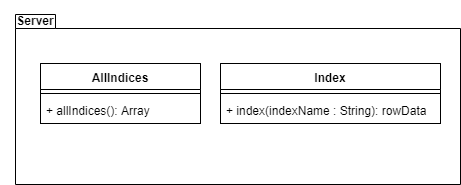
\includegraphics[width=1\textwidth]{Images/DiagrammaClassiServer.png}
	\caption{Diagramma UML delle classi riguardanti il lato server}
	\label{img:diagrammaClassiServer}
\end{figure}

\subsubsection{AllIndices}
AllIndices è la API che si occupa di restituire al chiamante la lista di \emph{tutti} gli indici presenti all'interno della istanza di Elasticsearch collegata. La lista degli indici è un array di stringhe contenente per ogni indice il proprio nome.

\subsubsection{Index}
Index è la API che espone l'interfaccia per poter leggere i dati contenuti all'interno di un indice. Nella richiesta GET deve essere specificato un parametro chiamato index, il cui valore rappresenta l'indice del quale si vogliono ottenere i dati. Ciò che viene ritornato al richiedente è un oggetto \emph{grezzo}, ovvero la risposta dell'istanza Elasticsearch, con tutti i dati amministrativi che Elasticsearch utilizza annessi (e.g. campi preceduti da underscore, \texttt{"\_id"}). Sarà compito del client reperire le informazioni a lui utili
